\chapter{Implementation}
\textit{In this chapter, we address the implementation phase of the project. After establishing a detailed analysis and a clear design, the implementation represents the concrete culmination of our work, through the deployment of the various components of the project. We will detail here the main steps, the tools used, the challenges encountered, as well as the solutions provided.}
\pagebreak

\section{Work Technologies}
\textbf{Java:}
Java was the primary programming language for the development of this project. Java was chosen for its robustness, portability, and extensive ecosystem, which make it suitable for building scalable and maintainable applications. Its strong type system and mature libraries contributed to reliable code, while its widespread adoption ensured access to a large pool of resources and community support.
\begin{figure}[H]
\centering

\includegraphics[width=0.2\textwidth]{img/tech/java-logo.png}
\caption{Java logo}
\end{figure}

\textbf{Spring Boot:}
Spring Boot is a framework that simplifies the development of Java applications by providing auto-configuration and embedded servers. It enables rapid development of production-ready applications with minimal configuration, while offering comprehensive features for dependency injection, security, and data access.
\begin{figure}[H]
\centering

\includegraphics[width=0.3\textwidth]{img/tech/springboot-logo.png}
\caption{Spring Boot logo}
\end{figure}

\textbf{PostgreSQL:}
PostgreSQL is an advanced, open-source relational database management system known for its reliability, feature robustness, and performance. It was used as the primary database for this project, providing ACID compliance, advanced indexing, and support for complex queries and data types.
\begin{figure}[H]
\centering

\includegraphics[width=0.2\textwidth]{img/tech/postgres-logo.png}
\caption{PostgreSQL logo}
\end{figure}

\textbf{Redis:}
Redis is an in-memory data structure store used as a database, cache, and message broker. In this project, Redis was utilized for caching frequently accessed data and session management, significantly improving application performance and reducing database load.
\begin{figure}[H]
\centering

\includegraphics[width=0.2\textwidth]{img/tech/redis-logo.png}
\caption{Redis logo}
\end{figure}

\textbf{Docker:}
Docker is a platform for developing, shipping, and running applications in containers. It ensures that the application runs consistently across different environments, simplifying deployment and scaling while isolating dependencies.
\begin{figure}[H]
\centering

\includegraphics[width=0.3\textwidth]{img/tech/docker-logo.png}
\caption{Docker logo}
\end{figure}

\textbf{GitLab:}
GitLab is a software development platform that allows developers to collaborate, manage version control, and store their projects using Git, a distributed version control system.
\begin{figure}[H]
\centering

\includegraphics[width=0.3\textwidth]{img/logos/gitlab-logo.png}
\caption{GitLab logo}
\end{figure}

\textbf{IntelliJ IDEA:}
IntelliJ IDEA is a powerful integrated development environment (IDE) for Java development. It was used throughout the project for code development, debugging, and refactoring, providing intelligent code completion, advanced debugging tools, and seamless integration with build tools and version control systems.
\begin{figure}[H]
\centering

\includegraphics[width=0.3\textwidth]{img/tech/IntelliJ IDEA.png}
\caption{IntelliJ IDEA logo}
\end{figure}

\textbf{Excalidraw:}
Excalidraw is a virtual whiteboard tool for creating hand-drawn-like diagrams and sketches. It was used in this project for creating wireframes, system architecture diagrams, and visual representations of workflows, facilitating better communication and planning among team members.
\begin{figure}[H]
\centering

\includegraphics[width=0.3\textwidth]{img/logos/excalidraw-logo.png}
\caption{Excalidraw logo}
\end{figure}

\textbf{Apache Kafka:}
Apache Kafka is a distributed event streaming platform used for building real-time data pipelines and streaming applications. It allows for the efficient handling of large volumes of data in real-time, making it suitable for applications that require high throughput and low latency.
\begin{figure}[H]
\centering

\includegraphics[width=0.2\textwidth]{img/tech/kafka-logo.png}
\caption{Apache Kafka logo}
\end{figure}

\textbf{Apache Avro:}
Apache Avro is a data serialization framework that provides compact, fast, binary data format with rich data structures. It was used in this project for schema evolution and data serialization in Kafka messages, ensuring efficient data transmission and backward compatibility.
\begin{figure}[H]
\centering

\includegraphics[width=0.2\textwidth]{img/tech/apache-avro-logo.png}
\caption{Apache Avro logo}
\end{figure}

\textbf{Confluent Schema Registry:}
Confluent Schema Registry is a centralized repository for managing and validating schemas for topic message data. It works seamlessly with Apache Avro to provide schema evolution capabilities and ensures data compatibility across different versions of applications consuming Kafka topics.
\begin{figure}[H]
\centering

\includegraphics[width=0.3\textwidth]{img/tech/CFLT_BIG.png}
\caption{Confluent Schema Registry logo}
\end{figure}
\newpage

\section{Technical Results:}


\subsection{Performance tests and quality measures}
In this section, we will present the performance tests and quality measures applied to the codebase and stateless worker in runtime. These tests are essential to ensure that the application meets the expected performance standards and adheres to best practices in software development.

\subsubsection{Load Testing}

Load testing is a critical aspect of performance evaluation, especially for applications that handle high transaction volumes. In this project, we conducted load tests to assess the application's ability to process transactions efficiently under varying loads. The tests were designed to simulate the expected transaction volume and measure key performance metrics such as CPU utilization, average processing time, and transactions processed per second.
The load testing was conducted using the xK6-kafka tool, which is specifically designed for load testing Apache Kafka applications. This tool allows us to simulate a large number of transactions and measure the performance of the application under stress. We chose xK6-kafka as an alternative to Apache JMeter due to its better support for Avro messages, which are used in our application.


\begin{figure}[h]
    \centering
    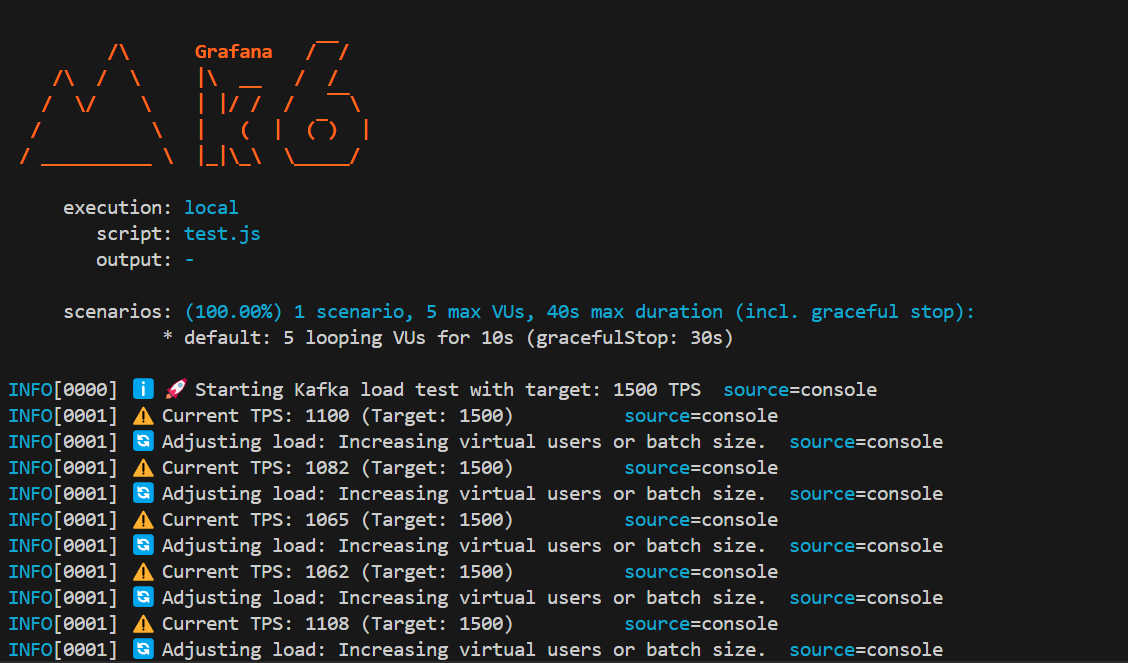
\includegraphics[width=1\textwidth]{metrics/k6-kafka-load-test.png}
    \caption{Load Testing Setup with xK6-kafka}
    \label{fig:load-test-setup}
\end{figure}


\begin{figure}[h]
    \centering
    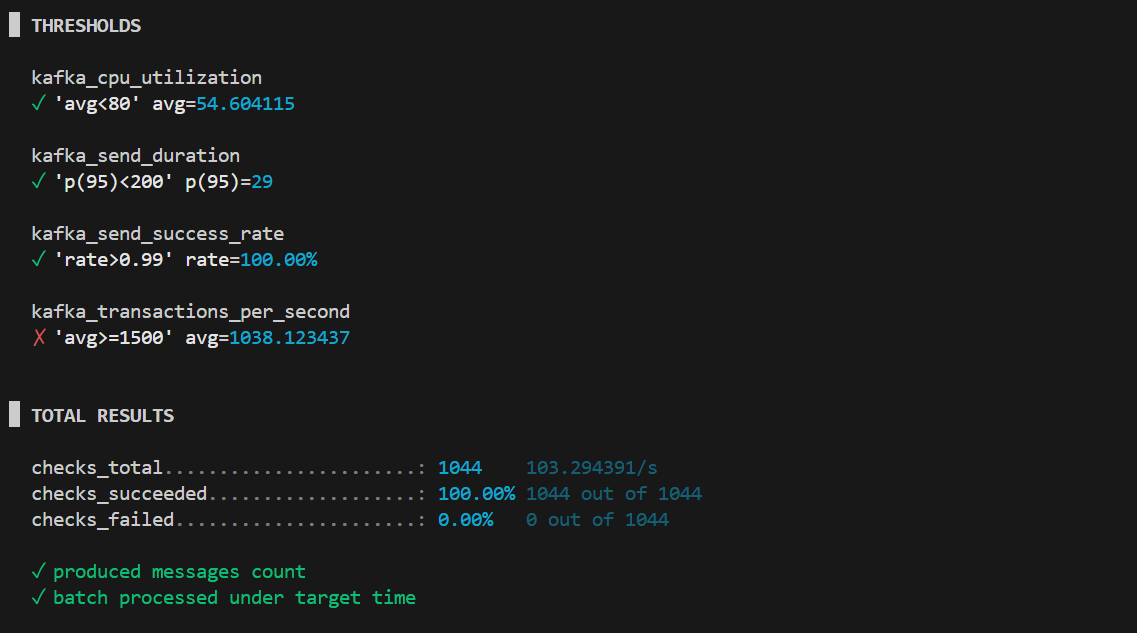
\includegraphics[width=1\textwidth]{metrics/k6-bilan.png}
    \caption{Load Testing Results}
    \label{fig:load-test-results}
\end{figure}

\begin{figure}
    \centering
    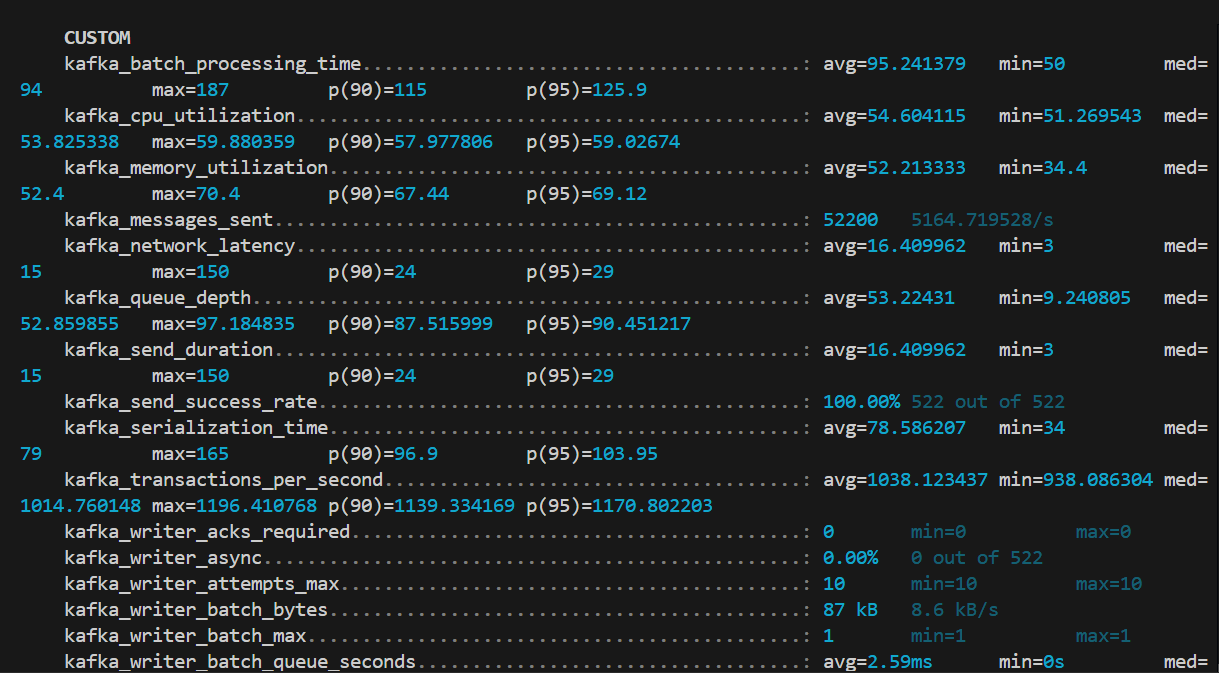
\includegraphics[width=1\textwidth]{metrics/kafka-metrics.png}
    \caption{Load Testing Results - Detailed Metrics}
    \label{fig:load-test-detailed}
\end{figure}

\FloatBarrier 
The load testing setup involved configuring the xK6-kafka tool to connect to our Kafka cluster and simulate a high volume of transactions. The tool was configured to send messages in Avro format, which is the format used by our application for transaction data.

The results captured during the load test are presented into the following table:

\begin{table}[h]
\centering
\caption{Kafka Producer Load Test Performance Results}
\label{tab:load_test_results}
\begin{tabular}{|l|c|c|c|}
\hline
\textbf{Performance Metric} & \textbf{Threshold} & \textbf{Achieved Result} & \textbf{Status} \\
\hline
CPU Utilization & avg $<$ 80\% & 54.60\% & \textcolor{green}{\checkmark} \\
\hline
Send Duration (P95) & P(95) $<$ 200ms & 29ms & \textcolor{green}{\checkmark} \\
\hline
Success Rate & rate $>$ 0.99 & 100.00\% & \textcolor{green}{\checkmark} \\
\hline
\multicolumn{4}{|l|}{\textbf{Additional Validation Metrics}} \\
\hline
Total Checks & - & 1044 & 103.29/s \\
\hline
Check Success Rate & - & 100.00\% & 1044/1044 \\
\hline
Message Processing & - & All batches & \textcolor{green}{\checkmark} \\
\hline
Batch Timing & $<$ 500ms & Under target & \textcolor{green}{\checkmark} \\
\hline
\end{tabular}
\end{table}



\subsection{Performance Analysis and Proof-of-Concept Validation}
The load test results demonstrate a \textbf{successful proof-of-concept implementation} with an achieved throughput of \textbf{1038.12 TPS}, representing \textbf{69.2\% of the target 1500 TPS goal}. While the absolute target was not reached, this performance baseline validates the fundamental architecture and identifies clear optimization pathways for production deployment.



\subsubsection{Proof-of-Concept Context and Limitations}
The current implementation operates with \textbf{multiple Kafka worker instances} deployed on a \textbf{single development server}, which inherently constrains the achievable throughput due to several infrastructure limitations:

\begin{itemize}
    \item \textbf{Resource Contention on Single Host}: Multiple worker instances (meta, context, ic, sf) compete for CPU, memory, and I/O resources on the same physical server, creating bottlenecks not present in distributed production environments.
    
    \item \textbf{Development Infrastructure Limitations}: Local server hardware specifications and network configuration do not reflect the high-performance, dedicated infrastructure available in production client environments.
    
    \item \textbf{Shared Resource Architecture}: All worker types sharing the same host creates resource contention and limits the ability to achieve optimal per-worker performance, unlike production deployments with dedicated resources per service.
    
    \item \textbf{Network Topology Constraints}: Local server deployment lacks the optimized network architecture, load balancing, and distributed infrastructure that production client environments provide.
\end{itemize}

In production client environments, each worker type would be deployed on dedicated, high-performance infrastructure with optimized resource allocation, enabling linear scaling and significantly higher throughput capacity.
\subsubsection{Positive Performance Indicators}
Despite not achieving the absolute TPS target, the results demonstrate several \textbf{critical success factors}:

\begin{itemize}
    \item \textbf{Perfect Reliability}: 100\% success rate with zero message loss validates robust error handling and transaction processing logic
    
    \item \textbf{Good Latency Profile}: P95 latency of 29ms (85\% better than 200ms threshold) indicates efficient message processing with substantial headroom
    
    \item \textbf{Efficient Resource Utilization}: 54.6\% CPU usage demonstrates the system operates well within capacity limits, suggesting potential for optimization rather than resource exhaustion
    
    \item \textbf{Stable Performance}: 100\% check success rate across all 1044 test iterations confirms consistent system behavior under sustained load
\end{itemize}




\textbf{Conclusion}: The proof-of-concept successfully validates the fundamental transaction processing pipeline architecture while identifying specific optimization vectors for achieving and exceeding production performance targets. The 1038.12 TPS baseline provides a solid foundation for confident production deployment with clear scaling strategies.

\subsubsection{Performance Optimization}
% Discuss optimizations made based on load testing results


\subsection{Deployment}
In this section, we will present the technical results of the project, focusing on the deployment of the application and the tools used to ensure its quality. 
The deployment process is crucial as it allows us to make the application available for use and to ensure that it meets the expected standards of quality and security.


\begin{figure}
    \centering
    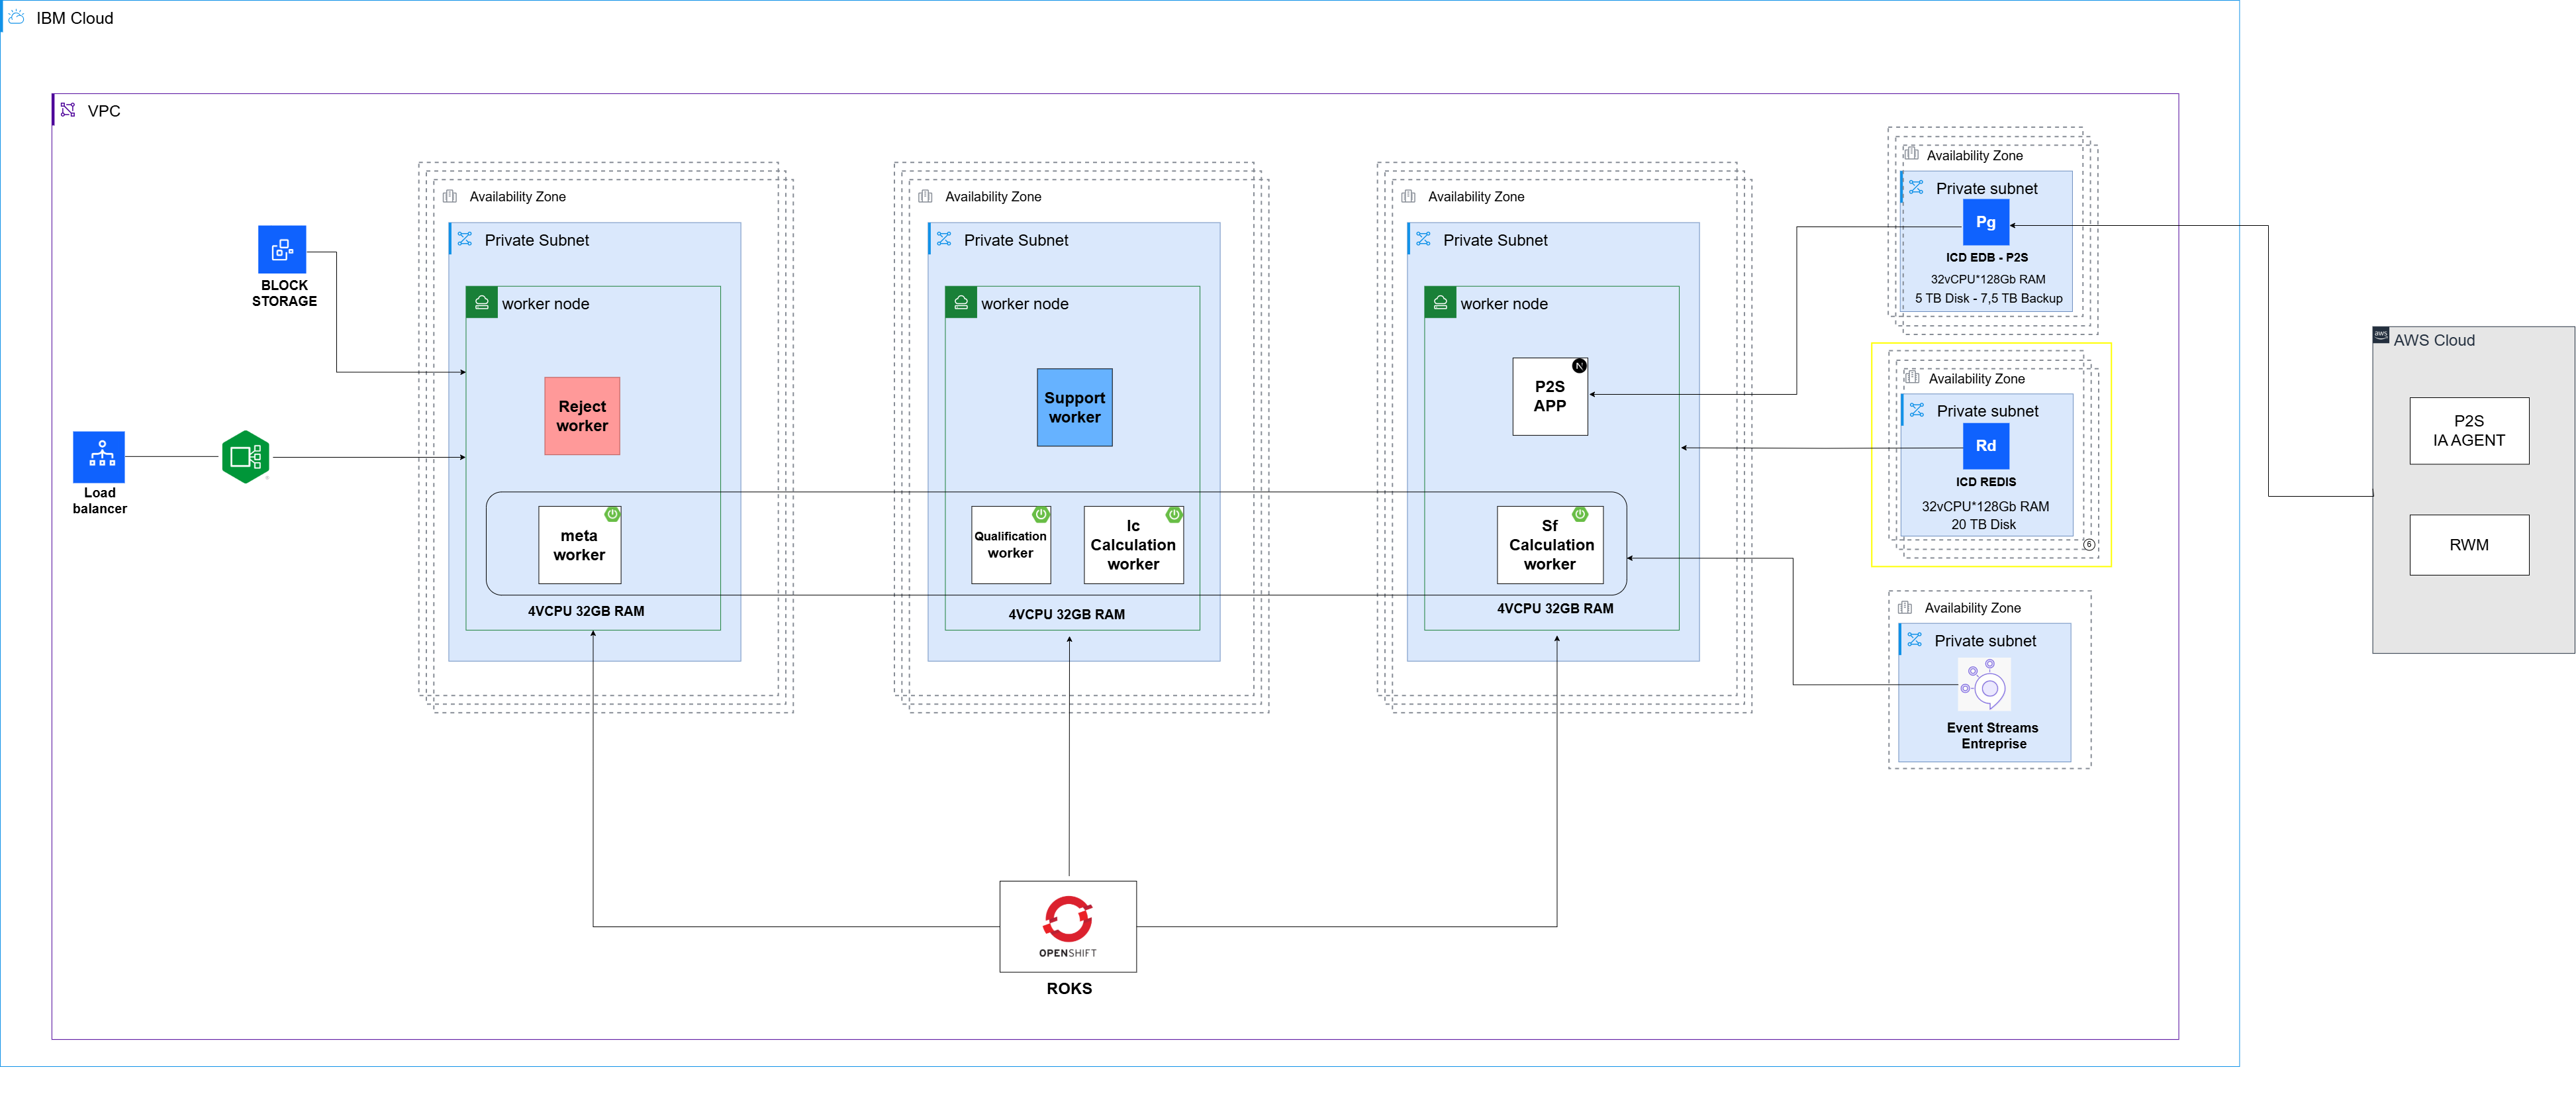
\includegraphics[width=1\textwidth]{img/arch/p2s-workers-deployment.drawio.png}
    \caption{Deployment Architecture}
    \label{fig:deployment}
\end{figure}
  
This architectural deployment demonstrates a distributed microservices approach optimized for high-availability transaction processing within IBM Cloud's multi-zone infrastructure. The system leverages  availability zones to ensure fault tolerance and geographic distribution, the compute engines deployed as instances in all availability zones as independent worker nodes provisioned with sufficient resources  to handle intensive financial calculations. 
The Meta Worker serves as the intelligent transaction dispatcher, while the second zone hosts the Context Qualification and Interchange Calculation engines responsible for transaction evaluation and fee computation. The third zone contains the Scheme Fees Calculation engine alongside the primary P2S application components.
This zonal distribution strategy ensures that critical processing components remain operational even during zone-level failures, while the stateless nature of each worker enables horizontal scaling based on transaction volume demands. The integration with ROKS (Red Hat OpenShift) provides container orchestration capabilities, while the Event Streams Enterprise implementation facilitates reliable Kafka-based messaging between components. The hybrid cloud approach, incorporating AWS services for extended P2S functionality, demonstrates the system's ability to leverage best-of-breed services across multiple cloud providers while maintaining centralized control within the IBM Cloud VPC infrastructure.




\section{Conclusion}
With this final step, we have completed the implementation of the project by applying the analytical and conceptual studies presented in the second chapter. We have presented the tools used for its development as well as the various interfaces that were created.
\pagebreak
